\documentclass[12pt, a4paper, openany]{report}
\usepackage[left=3cm, top=3cm, bottom=3cm, right=4cm]{geometry}

\usepackage{mystyle}
\usepackage{csquotes}

\pagestyle{fancy}
\fancyhf{}
\lhead{Partykomitee}
\chead{Spätes Theater}
\rhead{\thepage}

\title{
  {\textbf{Spätes Theater}}\\
  {\large{Eine Bildungsliverollenspielparty}}\\
  \bigskip
  \bigskip
  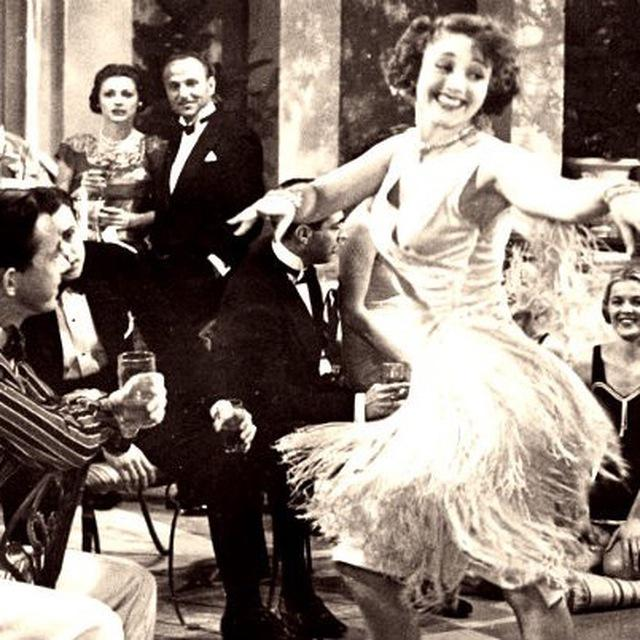
\includegraphics[scale=0.5]{titelbild.jpg}
}
\author{Tristan, Ronja, Anna, Jan}
\date{\today}

\begin{document}


\maketitle
\frontmatter
\tableofcontents
\mainmatter

\chapter{Einleitung}
\qq{Nur Arbeit und kein Spiel macht dumm} schrieb Karl Marx. 
\qq{Nur Arbeit und kein \emph{Feiern} macht ebenso dumm}, hätte er bestimmt genauso unterschieben. 
Über das Spiel und die Möglichkeit dabei zu lernen heißt es:
\qq{Es wird [...] \emph{ganzheitlich} gelernt: Kognitiv und affektiv, mit allen Sinnen, über Verstand, Körper und Gefühlen. 
Spielen ist ein Prozess -- nicht Ergebnis und Produkt, sondern der Ablauf selbst ist wichtig.}
Das gilt gleichermaßen fürs Feiern. 
Daher unser Konzept: 
Spielend Feiern! und dabei vielleicht auch ein bisschen lernen.

\chapter{Spielsetting}

\section{Zeitalter und Gepflogenheiten}

\section{Einladung für die Teilnehmenden/ Grund der Zusammenkunft}
Liebe Freunde und Vertraute,\\
wir leben in harten Zeiten. 
Um dies aufklären will ich dich klügsten Köpfe unserer Zeit zusammenrufen. 
Wir werden uns versammeln, um aufzudecken, wer die Protokolle der Weisen von Zion veröffentlicht hat. 

\chapter{Plot}

Alle Teilnehmer*innen werden von Baron Douleur eingeladen.


\section{Ronja}
Alle kennen den Veranstalter. 
Er hat großen politischen Einfluss. 
Am Anfang wird eine kurze Eröffnungsrede gehalten in der vier Leute vorgestellt werden, die als langjährige Vertraute des Veranstalters vorgestellt werden (vermutlich seine Diener).
Sie haben ein Projekt im Kopf und das wird im Laufe des Abends herumgetragen. 
Sie werden gleichzeitig durch den Abend die Gäste bewirtschaften und als Diener agieren.
Zwei davon sind gut und zwei insgeheim böse. 
Der Veranstalter weiß es nicht. 
Die Bösen wissen, wer dessen Verbündeter ist.
Die bösen haben somit einen Teamspieler. 
Im Verlaufe der Veranstaltung reden die vier Diener mit allen Gästen der Veranstaltung und versuchen sie für ihre Meinung zu gewinnen. 
Das soll son bisschen Werwolf-mäßig sein. 
Die Gäste müssen aus vorgeschriebenen Zetteln unterschreiben, auf denen ein konkreter Hinweis steht.
Z.B.: \qq{Wir sind gegen die Konzentration des Kapitals in den Händen von Hakennasen} (alternativ: \qq{von Puppenspielern})
Die Protokolle von Zion werden vorher kommuniziert. 
Beispielsweise dass wir dagegen sind, dass sich in bestimmten Händen kein Geld gelangen darf.\\

\section{Tristan}
Gehobene Veranstaltung von Wissenschaftlern, Künstlern, Politikern und Individuen.\\
Die Protokolle der Wissen von Zion sind entstanden wodurch die Juden als Böse Macht dargestellt werden. 
Die Gruppen der Veranstaltung arbeiten entweder für die Unterzeichnung dieser Protokolle oder dagegen.
Sollten sie unterschrieben werden werden böse und zerstörerische Interessen zur Wahrheit.
Wenn nicht, dann nimmt die Geschichte ihren Lauf und wir erreichen die uns bekannte Gegenwart.
Es geht also darum, die Vergangenheit so zu beeinflussen, dass alle zukünftigen Ereignisse geschehen können.
Beispiele: Relativitätstheorie wird entdeckt, Radioaktivität wird entdeckt, unglaubliche Kunstwerke entstehen, die unsere heutige Welt stark beeinflusst.\\
Sollten die Protokolle unterschrieben werden, würde die Jüdische Gemeinde als Böses Volk dargestellt.\\
Sollten sie nicht unterschrieben werden, würden sie inn Zukunft nicht gehasst werden und sie könnten Ihren Beitrag zur Weltgeschichte bringen.\\\\\\
Über den Verlauf der Veranstaltung laufen 4 Kellner herum, die Unterschriften für ein Dokument sammeln. 2 dieser Kellner sind neutral und 2 haben ein böses Motiv.
Alle Gäste

\qq{Wir sind gegen die Konzentration des Kapitals in den Händen von Hakennasen}

\chapter{Events}
\section{Präsentation}
\section{Tanzen}
Wir brauchen noch geile und passende Musik um zu tanzen:
Jazz, Swing z.B.

\section{Glücksspiel}
Eventuell als Verantwortliche : Michelle und Don

\section{Polizei-Besuch}
Zu einem bestimmten Zeitpunkt kommen die Bullen. (Evtl. ein Lied)

\chapter{Gruppen}
Die Gruppen sind als solche nicht mehr Bestandteil des Konzepts, stattdessen sollen Ziele vermehrt auf Einzelpersonen verlegt werden. 
Einzelne Beziehungs-Gruppen wird es evtl. immer noch geben. 
Hier bleiben Überbleibsel formuliert, die evtl. in Charaktere/ Beziehungs-Gruppe integriert werden. 

\section{Die Liebes Affäre}
\subsubsection{Backgroundstory}
\subsubsection{Hinweise für uns}
Vielleicht will diese Gruppe auch Menschen auseinander bringen.\\\\
Beispiel: Simone de Beauvoir (Frau von Sartre) mit jemandem verkuppeln\\
Beispiel: Love Triangle zwischen Nietzsche, Solomé und Rée
\subsubsection{Ziel}
Einige Charaktere wollen Character XY mit Charakter XZ verkuppeln.
Allerdings wollen ein bis drei Menschen dieser Gruppe Charakter XY mit Charakter XW verkuppeln.

\section{Politische Intrigen}
\subsubsection{Backgroundstory}
Diese Gruppe ist eine Linksradikale Gruppe.
\subsubsection{Ziel}
Diese Gruppe will, dass für einen Moment (z.B. während eines bestimmten Liedes) alle eine Maske tragen. 
Das will die Gruppe, weil sie weiß, dass zu dieser Zeit die Polizei kommt.
Währenddessen wollen sie daher unerkannt bleiben.

\subsubsection{Hinweise für uns}
Falls diese Gruppe ihr Ziel nicht erfüllt und die Polizei auftritt, ohne, dass alle die Masken tragen, bzw. ohne, dass erkenntlich ist, dass es sich um einen Maskenball handelt, werden sie festgenommen.
Dies verhindert letztendlich doch der Hausherr (\qq{das sind meine guten Freunde}), allerdings nimmt die Polizei ihnen ihr Stimmrecht entziehen (der Mechanismus fehlt noch; beispielweise könnte jede*r einen nicht personalisierten Stimmzettel besitzen, der ihnen dann abgenommen wird [diesen könnten sie dann leicht fälschen]). 

\subsubsection{Hinweise für uns}
\emph{Für diese Gruppe gibt es ein IT-Vortreffen, welches vor dem Spiel stattfindet.
Das Treffen soll ohne sozial Media o.ä. kommuniziert werden.}

\section{Weltherrschaft}
\subsubsection{Backgroundstory}
Möglicherweise ein grausiger Plan die Weltherrschaft zu übernehmen. 
Ein Haufen militärischer und dogmatischer unantastbarer Egozentriker (nein nicht Hitler) die mithilfe von machiavellistischen Mitteln die Weltherrschaft an sich reissen möchten. 

\subsubsection{Ziel}
Ihr Ziel ist es die geheimen Dokumente der Physiker zu erlangen, um die Baupläne für die Atombombe zu erhalten.

\subsubsection{Hinweise für uns}
Evtl. könnte diese Gruppe, um ihr Ziel zu erreichen, sich mit der Gruppe \qq{Seduction} zusammentun, um die abzufüllen.

\section{Atomskripte}
Dies ist keine wirkliche Gruppe im eigenen Sinne (wie die 4 zuerst genannten es sind). 
Es handelt sich um vier Wissenschaftler (Einstein, Planc, Heisenberg und Schrödinger), von denen jeder jeweils ein teil eines Skriptes zum Bau von Atomwaffen besitzt.
Diese Manuskripte, wollen andere Charaktere für sich nutzen (Beispiel: Gruppe Weltherrschaft).
Außerdem Herrschaft innerhalb der Gruppe ein Zwist: 
so haben Heisenberg, Schrödinger und Planc vor >>endlichen Jahren<< beschlossen sich in eine Irrenanstalt zurückzuziehen, um die Manuskripte vor der Öffentlichkeit zu schützen (siehe: Dürrenmatts >>Die Physiker<< [Ja, wir wissen, dass es sich dort um andere Personen handelt]).
Einstein, der ebenfalls eines der Manuskript-Teile besitzt, hat sich allerdings dagegen entschlossen, gleichfalls in die Irrenanstalt zu gehen.

\chapter{Charaktere}
Hier können wir alle Charaktere Versammeln.

\section{Figuren der Veranstaltung}
\begin{itemize}
   	 \item Butler
    	\item Diener
    	\item Veranstalter
\end{itemize}

\section{Mögliche Gast-Charaktere}
Vorschläge 
\subsubsection{Schriftsteller:innen}
\begin{itemize}
    	\item Ernest Hemingway (geboren 1899) (Seduction)
    	\item Jean-Paul Sartre (Poltische Intrigen)
    	\item Simone de Beauvoir (Politische Intrige)
    	\item Friedrich Nietzsche (Weltherrschaft)
    	\item Lou Andreas Salomé (Weltherrschaft)
    	\item Paul Rèe (Liebes Affäre)
\end{itemize}

\subsubsection{Wissenschaftler*innen}
\begin{itemize}
    	\item Newton (Kein Gruppe) 
    	\item Möbius (Keine Gruppe)
    	\item Albert Einstein (Weltherrschaft)
	\item Leibniz (Optimist) (Liebes Affäre)
	\item Sigmund Freud (Liebes Affäre)
	\item Marie Curie (Keine Gruppe)
\end{itemize}

\subsubsection{Künstler:innen}
\begin{itemize}
	\item Alfred Hitchcock (Seduction)
	\item Frieda Kahlow (Seduction)
	\item Salvadore Dalí (Seduction)
\end{itemize}

\subsubsection{Aktivist:innen}
\begin{itemize}
	\item Käthe Kollwitz (Politische Intriege)
\end{itemize}

\subsubsection{Andere Charaktere}
\begin{itemize}
	\item Enzo Ferrari (geboren 1898) (Weltherrschaft)
	\item Rudolf und Adolf Dassler (geboren 1998 und 1900) (Weltherrschaft)
	\item Gloria Swanson (Weltherrschaft)
\end{itemize}

\subsubsection{Politische Figuren}(Grundstein der Differentialrechnung)
\begin{itemize}
	\item Karl Liebknecht (Politische Intriegen)
	\item Rosa Luxemburg (Politische Intriegen)
\end{itemize}

\section{Charakterbeschreibungen}
Das sind die Beschreibungen, die die Teilnehmer:innen auch erhalten.

\subsection{Friedrich Nietzsche}
\subsubsection{Background}
\subsubsection{Psychologie}
\subsubsection{Politische Einstellung}
\subsubsection{Beziehungen}
\subsubsection{Deine Ziele}
Du willst Lou auf der Feier von Tristan einen zweiten Heiratsantrag machen.

\subsection{Lou Andreas Salomé}
\subsubsection{Background}

\textit{Geburt, Familie und Russland}\\
>>Ich bin Erinnerungen treu, Menschen werde ich es niemals sein.<< 
Das ist vielleicht dein heiligstes Motto, welches dich von Beginn an begleitete.
Am 12. Februar 1901%
\footnote{
  Lou Andres Salomé wurde eigentlich 1861 geboren. 
  Wir haben ihr Geburtsjahr 40 Jahre nach hinten verschoben, um es dem Setting unserer Geschichte anzupassen. 
  So verfuhren wir mit allen weiteren hier genannten Jahreszahlen.
}
wurdest du als jüngste Tochter und einziges Mädchen von sechs Kindern in eine wohlhabende, kulturell vielseitig interessierte Familie geboren. 
Du wuchst als Liebling deines Vaters, Gustav Ludwig von Salomé, auf. 
Dein Vater stammte von südfranzösischen Hugenotten ab und wurde während seiner militärischen Karriere, die ihn bis in den Generalstab der russischen Armee führte, durch Zar Nikolaus I in den Adelsstab erhoben.
Deine Mutter war norddeutscher-dänischer Herkunft. 
Sie heiratete deinen Vater 1884.

Bereits als Kind verweigertest du die Treue gegenüber Menschen, d.h.: auch gegenüber ihren Idealen:
du weigertest dich schicke Kleider zu tragen und an Bällen teilzunehmen, da du noch \qq{im Kampf um Gott} (so sollte dein späterer Debütroman getauft sein) standest, ließt du dich gleichfalls nicht konfirmieren und tratest aus der Gemeinde aus.
Dem ersten Menschen brachst du kurz vor deiner Abreise nach Zürich die Treue: 
ein 25 Jahre älterer Pfarrer, der dich in Philosophie unterrichtete und dir einen Heiratsantrag machte. 
(Aber vielleicht ist den Heiratsantrag eines Lehrers abzulehnen auch kein Bruch von Treue)
\medskip
\begin{center}
  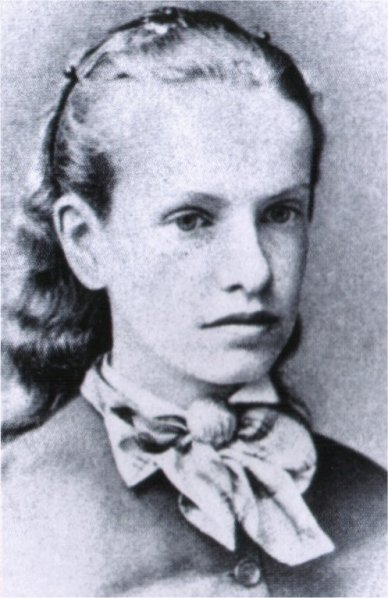
\includegraphics[scale=1.5]{Lou_profil.jpg}
\end{center}
\medskip
\textit{Zürich und Rom}\\
Nach Zürich reistest du gemeinsam mit deiner Mutter nach dem Tod deines Vaters (1918). 
Als Gasthörerin besuchtest du Vorlesung in Philosophie (Logik, Geschichte der Philosophie, Antike Philosophie und Psychologie) und Theologie. 
Die Universität Zürich war eine der wenigen Universitäten, die zu jener Zeit auch Frauen zum Studium zuließ.
Wenig später, empfahl ein Arzt dir den Aufenthalt in einem wärmendem Klima, um dort ein Lungenleiden auszukurieren. 
1922 trafst du in Rom ein, wo du mit Hilfe eines Empfehlungsschreibens Zugang bekamst zu einem Kreis um die Schriftstellerin, Pazifistin und Frauenrechtlerin Malwida von Meysenbug.
Zu dieser Zeit entwickeltest du neben Interessen an der Philosophie und Theologie auch ein Interesse an der Literatur und dem eigenen Schreiben. 
Du versuchtest dich zu nächst ein Lyrik, und ein wenig später ab noch in deiner Rom-Zeit entstanden erste Versuche kürzere Prosa. 
In Malwidas Bekanntenkreis verkehrt auch der junge Philosoph Paul Rée, zu dem du umgehend freundschaftliche Gefühle aufbautest, während er sich in dich umgehend verliebte und dir einen Heiratsantrag machte, den du -- natürlich -- ablehntest. 
Wenig später machte Rée dich mit seinem Freund Friedrich Nietzsche bekannt, der ebenfalls aus gesundheitlichen Gründen nach Rom reiste. 
Friedrich Nietzsche war Professor für klassische Philologie an der Universität Basel, doch seine Migräne und Magenleiden ließen ihn seine Professur aufgeben. 
Auch er verliebte sich sofort in die >>junge Russin<<, in dich, auch er machte dir einen Heiratsantrag und auch diesen lehntest du ab.
\\
\\
\textit{Ménage à trois}\\
Du hattest anderes im Sinn: 
Dir schwebte eine >>ménage à trois<< vor -- ganz ohne Sex, eine rein platonische Wohngemeinschaft zu dritt.
Dein Wunsch war eine Künstler*innen und intellektuellen Zuflucht, sowie eine Arbeitsgemeinschaft: die von dir sogenannte >>Dreieinigkeit<<.
Diesen gemeinsamen Zufluchtsort, errichtetet ihr euch in der Nähe von Wien, wo ihr freundschaftlich zusammenleben, studieren, schreiben und diskutieren solltet.%
\footnote{
  Diese Wohngemeinschaft wurde zwar lange geplant, kam aber in Wirklich nie zustanden. 
  Sie zerbrach neben der Eifersucht Nietzsches und Rées auch an den Bemühung Nietzsches Schwester, die Andreas-Salomé für einen schlechten Einfluss hielt.
}\\
Natürlich schien es für manche Menschen eine unerhörte Sache zu sein, drei unverheiratete Menschen zusammenwohnen zu sehen, dazu meintest du mal:
\begin{itemize}
  \item[] \emph{\qq{Wir wollen doch sehn, ob nicht die allermeisten sogenannten >>unübersteiglichen Schranken<< die die Welt zieht, sich als harmlose Kreidestriche herausstellen!}}
\end{itemize}
Deine Freundschaft mit Paul Rée gedieh in eurem gemeinsamen Haus weiter und war relativ unkompliziert, obwohl du seine Liebe dennoch spürtest. 
Ihr wurdet vertrauter miteinander, schicktet euch Tagebuchblätter zu und beriet euch über den jeweiligen Stand der Dinge im Verhältnis zu Nietzsche, der von alledem nichts wusste. 
Obwohl du Nietzsche als Philosophen, Freund Lehrer und Gesprächspartner sehr schätztest, wurde eure Beziehung zunehmend kompliziertet:
nicht nur erdrückte dich seine Liebe und Eifersucht, die er zwar nicht offen zu zeigen versuchte, die dir aber dennoch im gegenwärtig war, auch bekamst du mit, dass seine Schwester Elisabeth Förster-Nietzsche, von eurer Wohnsituation alles andere als begeistert war.
So stellte seine Schwester, die teilweise über Nietzsches Diäten der Basler Universität verfügte, die Zusendung der notwendigen Gelder ein.
\\
\\
\textit{Berlin}\\
Da die Veröffentlichung Nietzsches nächsten Werkes noch einige Zeit dauern sollte, beschlosst ihr gemeinsam, dass Nietzsche und du nach Berlin reisen solltet, um dort an ein wenig zusätzliches Geld zu kommen, während Rée sich um die Angelegenheiten in eurem Haus bemühen sollte.
Ihr bezogt eine kleine Wohnung im Zentrum von Berlin. 
Das blühende, extravagante und freizügige Leben in Berlin zog dich sofort in seinen Bann. 
Die vielen Feiern in der Stadt und in den intellektuellen und wohlhabenden Kreisen stellten sich bald als hervorragende Möglichkeit etwas zu verdienen und zugleich neue Verbindungen zu knüpfen da:
ihr arbeitetet als Kellner auf verschiedenen Feierlichkeiten und erhieltet dort die Möglichkeit die einflussreichen Menschen der Stadt kennenzulernen. 
Viel und oft wart ihr bei Feiern von Herrn Tristan eingeladen, der euch bald gerne einstellte, gut bezahlte und einer menge Menschen vorstellte.

Für Nietzsche war der gemeinsame Aufenthalt eine Möglichkeit sich dir besonders verbunden zu fühlen, gleichzeitig rieb ihn jedoch das Leben in der großen Stadt, auf engen Raum und stets umgeben von einer so großen Anzahl an Personen auf. 
Schnell schon schlug er vor, auf eure Residenz zurückzukehren. 
Du jedoch wolltest gerne länger bleiben.
Du hattest auf einer Ausstellung die Künstlerin Frida Kahlow kennengelernt, und obwohl ihr an dem Abend nicht mehr als ein paar Sätze und eure Adressen austauschtet, spürtesttest du zum ersten Mal zu einer Person mehr als nur dieses Bedürfnis nach platonischen Freundschaft. 
Aus einem kurzen Briefwechsel erfuhrst du, dass sie auf der bald stattfindenden Feier von Herrn Tristan anwesend sein würde. 
Du überzeugtest Nietzsche noch ein wenig länger zu bleiben, um zumindest auf dieser Feiern noch ein Mal zu >>arbeiten<<.

\subsubsection{Psychologie}
\begin{center}
  \textit{
    >>Warst mir die müttlerlichste der Frauen\\
    ein Freund warst Du, wie Männer sind,\\
    ein Weib, so warst Du anzuschauen,\\
    und öfter noch warst Du ein Kind.\\
    Du warst das Zarteste, das mir begegnet,\\
    das Härteste warst Du, damit ich rang.\\
    Du warst das Hohe, das mich gesegnet -\\
    und wurdest der Abgrund, der mich verschlang.<<\\
  }
  \medskip
  -- Rainer Maria Rilke.\\
\end{center}
So wurde ich von jemandem beschrieben? 
Ein Kind bin ich vielleicht, ja.
Und das Höchste bin ich! 
Jedenfalls verlangt es mich danach und es treibt mich dort hin.
Und eine Mutter bin ich und will es auch sein, wenn ich das Gefühl habe Mutter für das Hohe zu sein. 
Aber ich stoße es ab, wenn Mutter für etwas sein mich davon abhält meinen Weg zu gehen. 
Dann bleibt wird es für mich zur und bleibt als Erinnerung. 
Ich frage mich, ob es mit Nietzsche so verlaufen wird. 
Vielleicht nichtmal nur um meinetwillen, sondern auch um seinetwillen. 
Wenn ich sehe, wie sich durch mich in ihm Triebe entwickeln, die seinem Wesen entgegenstehen... -- dann ekelt es mich, so könnte ich beinahe sagen, an.
Daher spricht das Gedicht war:
ich bin als Wein \emph{anzuschauen} den kein Weib vermag es sich so von allem emanzipieren zu \emph{wollen}, wie ich es will, wie ich es tue.
Daher bin ich weniger solidarisch mit dem Weib, sondern eher und vor allem solidarisch mit mir.
\bigskip
\begin{center}
  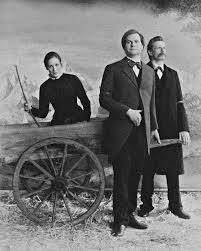
\includegraphics[scale=0.7]{lou.jpeg}
\end{center}
\subsubsection{Politische Einstellung}
\subsubsection{Beziehungen}
\subsubsection{Deine Ziele}
Du musst dringen noch einen Brief an Paul Rée verfassen, dem du viel zu lange nicht mehr geschrieben und außer dem versprochen hattest dich bis zum Ende der Woche bei ihm zu melden. 

\newpage


\subsection{Albert Einstein}
\subsubsection{Background}
\begin{itemize}
\item Anhänger des Judentum, Kämpfer gegen die Naziherrschaft
\item 14. März 1879 als erstes Kind von Hermann und Pauline Einstein in Ulm geboren
\item Jüngere Schwester Maja
\item Harmoniegetriebenes, liberales Umfeld
\item Als Kind viel umgezogen, deswegen vertraut er Menschen nicht so einfach und ist sehr aufmerksam, was andere Menschen tun.
\item In der Schule hatte er viele Probleme und konnte nie den Anschluss finden sowohl mit den Schülern, als auch mit dem Lehrstoff
\item Seine Studienzeit ist von Langeweile geprägt, für ihn ist das alles zu primitiv und einfach
\item Seine Aufmerksamkeitsspanne für das was man ihm sagt, ist sehr kurz
\item 1906 wird ihm der Doktorgrad verliehen, die Arbeiten bringen ihm 1921 auch den Nobelpreis ein
\item Frau Mileva Maric betrog er in Berlin er eine Affäre mit seiner Cousine Elsa Einstein Löwenthal beginnt
\item später veröffentlicht er seine Allgemeine Relativitätstheorie 
o	Mit dieser wird er 1919 schlagartig berühmt und rückt ins Rampenlicht der Weltöffentlichkeit
\item Mit seiner Popularität steigen allerdings auch die Anfeindungen gegen ihn - besonders von rechter Seite
\item Als in Deutschland der Ruf nach einem "starken Mann an der Macht" lauter wird und öffentliche Anfeindungen gegen Einstein an der Tagesordnung sind, beschließt er Deutschland den Rücken zu kehren und 1932 in die USA auszuwandern. Er blieb dabei sehr lang unter harten Bedingungen und erheblichem Risiko in "Barbarien" leben. Es gab offene Aufrufe zum Mord: "Zur Liga gehören u.a. Professor Einstein.... Wir würden jeden Deutschen, der diese Schufte niederschießt, für einen Wohltäter des deutschen Volkes halten," musste Einstein in der "Staatsbürger- Zeitung" lesen
\item er führt seit Jahren eine Brieffreundschaft mir Marie Curie aber hatte sie zuvor noch nie getroffen. Sie schrieb ihm aus akademischer Verehrung und Bewunderung, woraus schnell eine schriftliche Affäre wurde, die Albert Einsteins Ego nährte.
\end{itemize}

\subsubsection{Psychologie}
\begin{itemize}
\item Sein Gott war vielmehr ein Prinzip - das von Ursache und Wirkung (Kausalitätsprinzip Newtons)
\item In seiner Religion ist er gut aufgewachsen, aber ist keinesfalls streng religiös
\item Für ihn geht es um harte Arbeit, weil von nichts kommt auch nichts
\item Einstein war schlichtweg gemein und weder seine Familie noch seine Freunde konnten seine unberechenbaren Launen vorhersehen
\item Einzelgänger
\item Frauenverachter, viele Affären
\end{itemize}


\subsubsection{Politische Einstellung}
\begin{itemize}
\item Deutschen bist du sehr skeptisch gegenüber
\item Er ist ein Kind der Logik 
\item Linksliberal (?)
\item "Wir müssen uns unserer Artfremdheit klar bewusst sein und aus ihr die Konsequenzen ziehen. Es hat keinen Sinn zu versuchen, die anderen von unserer seelischen und geistigen Ebenbürtigkeit überzeugen zu wollen, denn die Wurzel ihres Verhaltens sitzt nicht im Großhirn."
\item ''Ich verachte alle, die es lieben im Takt der Musik zu marschieren, denn sie haben ihr Gehirn nur aus Zufall bekommen, ein Rückgrat hätte dazu vollkommen gereicht."
\item Im Exil regte er den Bau der Atombombe an, um Deutschland zuvorzukommen.
\end{itemize}

\subsubsection{Beziehungen}
\subsubsection{Deine Ziele}
\begin{itemize}
\item den Nazis alle Macht entziehen
\item ...
\end{itemize}

\subsection{Isaac Newton}
\subsubsection{Background}
\begin{itemize}
\item geboren 1643
\item aufgewachsen bei seiner Großmutter in Woolsthorpe (England)
\item Er arbeitete vor allem an den Problemen der Optik, der Algebra und der Mechanik
\item Welche Sprache spricht Newton und gibt es eventuelle Sprachbarrieren bspw. mit Möbius?
\item Lebte zur Zeit der Pest, Pandemie in England zwischen 1665 und 1666
\item to destroy the reputation of Gottfried Leibniz, who he believed (quite unfairly) had stolen the discovery of calculus from him 
\end{itemize}

\subsubsection{Psychologie}
\begin{itemize}
\item war sehr emotional. Streitereien oder Kritik an seiner Arbeit gingen ihm sehr nahe.
\item Hat von Zeit zu Zeit Nervenzusammenbrüche 
\item Nach dem Tod seiner Mutter wird Newton zum Einzelgänger
\item In Hinsicht auf  Wissen war newton nimmersatt
\item Vertraut anderen nicht leicht und hat kaum bis keine engen Freunde \\bis auf Möbius, der sein akademischer Vertrauter ist
\item Viele Menschen in einem Raum überfordern ihn und lassen ihn zumeist verstummen
\item Da er bei seiner Großmutter aufgewachsen ist, hat er eine sehr feminin geprägte Erziehung genossen und ist dementsprechend nicht gut auf schlechte Behandlung von Frauen zu sprechen. Beispielsweise würde er laut werden, wenn Einstein Marie Curie beleidigt, wird er auf einmal laut
\item Gibt es bei ihm einen unterschwelligen Judenhass, der sich ggf. auf Einstein auswirken kann?
\end{itemize}

\subsubsection{Beziehungen}

\subsubsection{Politische Einstellung}
\begin{itemize}
\item sehr in seinem akademischen Kreis gefangen
\item weiteres Umfeld gleichgültig
\item ...
\end{itemize}
\subsubsection{Deine Ziele}

\subsection{Möbius}
\subsubsection{Background}
\begin{itemize}
\item Charakter Möbius kann zu Teilen aus Möbius die Physiker, Willy Möbius und einem weiteren Charakter zusammengestellt sein
\item Er war zu Anfang in der Geschichte der Physiker der Mittelpunkt doch nun ist er nur einer von dreien und dazu kommt, dass er der unbekannteste von allen ist
\end{itemize}

\subsubsection{Psychologie}
\begin{itemize}
\item aufgrund seiner Erfolgslosigkeit wurde er zum verbitterten Alkoholiker
\item er versucht sein Unglück zu verbreiten, damit er sich nicht mehr allein fühlt und versucht Newton mit in sein Loch zu ziehen.
\end{itemize}
\subsubsection{Politische Einstellung}
\subsubsection{Beziehungen}
\subsubsection{Deine Ziele}

\subsection{Marie Curie}
Dein voller Name ist Marie Skłodowska Curie. Du wirst 1867 in Warschau geboren, ziehst jedoch nach Frankreich, da Frauen in Polen nicht zum Studium zugelassen wurden. Später wurde bei deinen wissenschaftlichen Erfolgen gerne verschwiegen, dass du polnische Herkunft hattest.
Selbst in Paris waren damals von 9000 Studenten nur 210 Frauen. Deine Familie wollte ein Auslandsstudium für dich nicht finanzieren daher erarbeitetest du dir das Geld selber, indem du Privatunterricht gabst.\\
Du bist Physikerin und Chemikerin und untersuchst hauptsächlich die beobachtete Strahlung von Uranverbindungen. Damit prägst du den Begriff der \qq{Radioaktivität}. Mit dieser Forschung wirst du so bekannt, dass du einen anteiligen Nobelpreis gewinnst sowohl für Physik als auch für Chemie. Hierbei arbeitest du viel mit deinem Ehemann zusammen, der die gleichen Forschungsschwerpunkte hat wie du. Nach dem tragischen Unfalltod deines Mannes kommst du zunächst seiner Lehrverpflichtung nach und unterrichtest später an einem Lehrstuhl für allgemeine Physik. Damit warst du die erste Professorin deiner Universität und prägst die weitere Forschung für Frauen. \\

An der Universität bist du neben deiner Forschung zudem politisch aktiv und lernst hier auch Simone de Beauvoire und Jean-Paul Sartre kennen. Hieraus entsteht eine langjährige Freundschaft. Auch wenn du Sartre an sich ganz nett findest, ist er doch eher der Lebensgefährt von Simone für dich und die eigentliche Freundschaft spielt sich eher zwischen euch beiden ab.\\

Zudem hegst du eine langjährige Brieffreundschaft mit Einstein, jedoch habt ihr euch nie persönlich kennen gelernt, werdet dies jedoch auf der Party das erste mal tun. 

\subsubsection{Background}

\subsubsection{Psychologie}

Seit dem Verlust meines Mannes leide ic hunter starken Depressionen. Eine Freundschaft wie mit Simone hilft mir an andere Dinge zu denken.
\subsubsection{Politische Einstellung}
Politisch bist du besonders daran interessiert das Studium an Universitäten für Frauen zu erleichtern. Hier setzt du dich sehr für ein und hast daher auch viele parallelen mit deiner Freundin Simone. 
\subsubsection{Beziehungen}
\subsubsection{Deine Ziele}

\subsection{Simone de Beauvoire}
 
\subsubsection{Background}

\qq{Wenn man uns sagt: ‚Immer schön Frau bleiben, überlasst uns nur all diese lästigen Sachen wie Macht, Ehre, Karrieren, seid zufrieden, dass ihr so seid: erdverbunden, befasst mit den menschlichen Aufgaben ‘ Wenn man uns das sagt, sollten wir auf der Hut sein!}

– Simone de Beauvoir\\


Deine Rolle in diesem Spiel ist Simone de Beauvoire. Falls dir der Name noch nichts sagt, lass mich dir einbisschen auf die Sprünge helfen und etwas über deine Geschichte erzählen. 
Dein vollständiger Name ist Simone-Lucie-Ernestine-Marie Bertrans de Beauvoir und du wirst 1908 in Paris geboren. Du erlangst einen großen Bekanntheitsgrad als Schriftstellerin, Philosophin und an der Seite deines Lebensgefährten Jean-Paul Sartre. Deine Philosophie dreht sich, ebenfalls wie die deines Lebensgefährten, um den Existentialismus. Zudem schreibst du mit deinem Buch \qq{Das andere Geschlecht} einen der bedeutsamsten Romane für die feministische Literatur, welcher dich zu eine der bedeutsamsten Intellektuellen Frankreichs macht. \\

Deine Familie verarmt während des Krieges. Daher musst du dich schon früh damit auseinander setzten für dein eigenes Geld zu sorgen, was du hinsichtlich jeglicher Erwartungen eher als einen Segen empfindest. Dein schöpferischer Freigeist fängt an sich zu entfalten und du entwickelst dein eigenes Idealbild von dir selbst, welches dich als ständig Lernenden und Erschaffenden Frau sieht. Von dem Bild der klassischen Hausfrau distanzierst du dich immer weiter. Du verlierst schon früh den Glauben an Gott und spielst deine scheinheilige Frömmigkeit über viele Jahre, bis du schließlich offen zu deinem Atheismus stehst. \\

Nachdem du von einer katholischen Mädchenschule als Musterschülerin abgehst, beginnst du dein Studium in Paris im Fach Philosophie, wo du auch Sartre und deine Langjährige Freundin Marie Curie kennen lernst. Du bist weiterhin Kirchlich aktiv um das Gemüt deiner strengen Eltern etwas zu besänftigen. Mit deinem ersten Verdienst durch das Lehren treibst du dich viel in Bars herum und lernst das verruchte Pariser Nachtleben immer besser kennen. \\

Bei der Agregation (kompetitive Prüfung innerhalb Frankreichs) belegst du den 2. Platz hinter Sartre. So sollte es dein Leben lang auch bleiben. Immer die zweite, immer die Lebensgefährtin von Sartre. Nie als erste genannt zu werden, nicht als Frau, nicht als Künstlerin, nicht als Philosophin. Doch dies ändert sich mit der Einladung zu dem \qq{Ball von Tristan}. Du wirst als wichtiges Mitglied der Intellektuellen angesehen und deine Meinung als Entscheiderin wird gefragt. Dein Lebensgefährte wiederum wird bei den Einladungen ausgelassen und begleitet dich somit nur. Diesmal ist Sartre die +1 nicht mehr du. Du merkst wie unangenehm Sartre die Situation ist und versuchst den Ruhm nicht zu sehr auszukosten, innerlich triumphierst du jedoch über die Situation \\

Deine Beziehung zu Sartre ist von lockerer und offener Natur. Die von ihm angebotene Heirat lehnst du ab, ihr bleibt jedoch weiterhin ein Paar. Ihr habt beide nebenbei immer wieder Liebschaften mit anderen Personen, in deinem Fall mit Männern und Frauen. Deine Bücher haben häufig Autobiographische Neigungen in denen du die Beziehung zu Sartre und anderen Liebschaften verarbeitest. \\

Mit deiner Freundin Marie-Curie verbindet dich der weibliche starke Freigeist. Du lernst sie in einem politischen Seminar an der Uni kennen und ihr versteht euch obwohl eure Forschungsansätze so unterschiedlich sind, von Anfang an gut.  



\subsubsection{Psychologie}

Ich durchlebe mein Leben lang innere Konflikte und depressive Phasen, die sich damit auseinandersetzten, kein anständiges, braves, bürgerliches Mädchen zu sein. Der innere Kampf zerreißt mich fast. Erst nachdem sich meine Werke immer besser verkaufen kriege ich genug Support meine Rolle immer weiter und mit mehr Selbstbewusstsein auszuleben. \\ 
Mein Liebesleben fühle ich lange als bedrückend und einnehmend. Ich möchte mich von dem  herrschenden, konservativen Ideal einer Frau lösen und meine Freiheit sowohl sexuell als auch beruflich ausleben. Gleichzeitig bin ich in einer erdrückenden Liebesbeziehung mit Sartre, welcher mich immer als Mann dominieren wird. Ich werde es nie schaffen mich von ihm zu lösen und ihn zu dominieren und habe mich mit dieser Tatsache eigentlich abgefunden, denn trotzdem liebe ich ihn und wir lassen uns viele Freiheiten.
Wenn ich nur die gleichen Rechte wie ein Mann hätte und mich so ausleben könnte, in einem anderen Körper geboren. Gleichzeitig liebe ich den weiblichen Körper und meine daraus entstehende Stärke und möchte mich nur von bestehenden Stigmata entfernen. Meine Freundin Marie Curie bewundere ich dafür, dass sie sich von dem Schatten ihres Mannes lösen konnte und mit ihrer eigenen Forschung bekannt wurde. Auch wenn ich grundlegend nicht an Naturwissenschaften interessiert bin, wird sie immer ein Vorbild für mich sein und dafür liebe ich sie. 



 
\subsubsection{Politische Einstellung} 

Der aufkeimende Nationalsozialismus beschäftigt dich. Somit sprichst dich zusammen mit Sartre und vielen anderen Intellektuellen klar dagegen aus und versuchst den Widerstand voran zu treiben. Sartre und du gründet eine Widerstandsgruppe mit dem Namen \\q{Sozialismus und Freiheit} um gegen den Faschismus weiter vorzugehen. Sartre und du steht zudem für die Gründung eines jüdischen Staates ein, der von der UNO militärisch geschützt werden soll. \\

Ebenfalls zusammen mit Sartre bist du starker Überzeugung und Mitbegründerin des Existentialismus. Der Existentialismus \qq{erklärt, dass es mindestens ein Wesen gibt, bei dem die Existenz der Essenz vorausgeht, ein Wesen das existiert, bevor es durch irgendeinen Begriffe definiert werden kann und das dieses Wesen der Mensch ist.} Das bedeutet, \qq{dass der Mensch zuerst existiert, sich begegnet, in der Welt auftaucht und sich danach definiert}. Danach ist Mensch darum nicht definierbar, weil er anfangs überhaupt nichts ist. Er wird erst in der weiteren Folge sein, und er wird so sein, wie er sich geschaffen haben wird. Der Mensch ist lediglich so, wie er sich will und wie er sich nach der Existenz konzipiert der Mensch ist nichts anderes, als wozu er sich macht. Über diese Themen unterhältst du dich gerne und viel, besonders mit Sartre und lässt es neben dem Feminismus immer wieder in deine Bücher einfließen. Die Kernthese vorausgesetzt, besagt dies jedoch, dass der Mensch die volle Verantwortung für das trägt, was er ist. Vor allem findet er keine Entschuldigungen, z.B. durch die Natur (à la der Mensch ist eben so) – Er ist für all sein Handeln voll verantwortlich. 




\subsubsection{Beziehungen}

\subsubsection{Deine Ziele}

Dein Ziel ist es die Philosophie des Existentialismus immer weiter zu verbreiten. Daher hast du als Aufgabe drei Personen (muss noch ausgewählt werden) von deinen Theorien zu unterrichten. Als frühere Lehrerin liegt dir das unterrichten und verbreiten von deiner Kunde quasi im Blut. Zudem bist du fest überzeugt, wenn Leute dem Existentialismus mehr Gewicht beiliegen würden, der immer stärker aufkommende Faschismus keine Chance hat Überhand zu gewinnen.

\subsection{Jean Paul Satre}
\subsubsection{Background}
\subsubsection{Psychologie}
\subsubsection{Politische Einstellung}
\subsubsection{Beziehungen}
\subsubsection{Deine Ziele}
Sartre versucht als Mießepeter allen was zu versauen...



\subsection{Salvador Dali}
\subsubsection{Background}
\begin{itemize}
\item Vollständiger Name: Salvador Felipe Jacinto Dalí y Domenech Fürst von Schmetternich
\item Mudda-Komplex
\item scharfe Erziehung von seinem Vater, Schlechte Beziehung somit zu Männern
\item Fühlt sich bei Frauen geborgen 
\item Hatte einen älteren Bruder, der früh starb und eine jüngere Schwester
\item entwickelte sehr früh eine starke Affinität zur Kunst
\item Beide Elternteile unterstützten seine Kunst und seinen Werdegang als Künstler
\end{itemize}

\subsubsection{Psychologie}
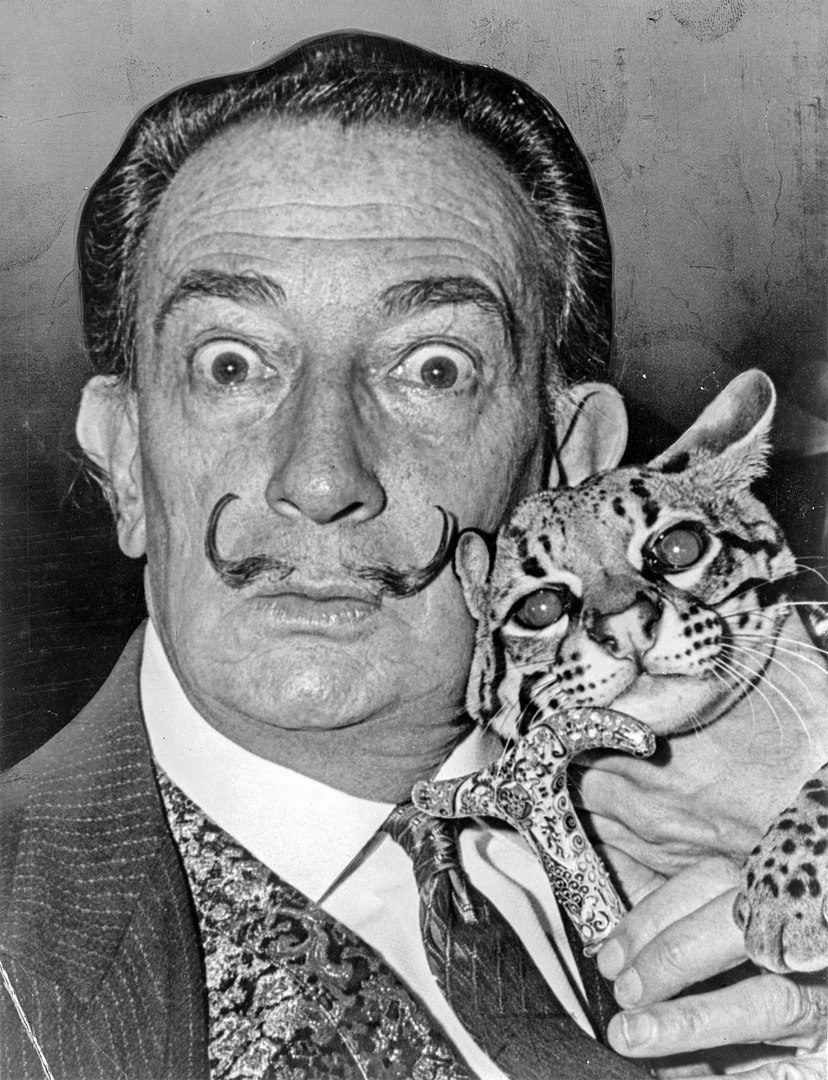
\includegraphics[width=8cm]{Salvador-Dali.jpg}\\\\
Extrovertierte crazy person mit einem leo fetisch.  Vielleicht auf LSD hängen geblieben. Denkt dass er immer klüger ist, als die Personen die im gegenüber stehen und berichtigt gerne.

\begin{itemize}
  \item In Katalonien geboren und groß geworden
  \item Aussenseiter unter den Surrealisten aufgrund politischer Richtung
  \item Extrovertierter Künstler
  \item hält sich für etwas besseres als viele Andere
  \item komischer Vogel
  \item Schnurrbart/Schnauzer war wichtig für sein Image, bekannt dafür bis in die heute Zeit
  \item suchte den Zustand der Paranoia um seine Kunst voll zu verkörpern
  \item bezahlte Essen und Getränke mit Kunst, möglicherweise bezahlt er seine Getränke auf Veranstaltungen mit Skizzen seine Ideen
  \item Sehr stark von Mode inspiriert und arbeitete auch mit Persönlichkeiten aus der Modewelt zusammen
  \item seltsame intellektuelle, jedoch intensive Liebesbeziehungen 
  \item Sehr von sich selbst überzeugt, eigenwilliger Charakter, 
  \item Kunst stammt aus der Welt des Traumes, Surrealismus
\end{itemize}

\subsubsection{Politische Einstellung}

\subsubsection{Beziehungen}

\subsubsection{Deine Ziele}

\chapter{Gruppenbeschreibung}

\subsection{Einstein, Newton,...}
Vor vielen Jahren haben sich die drei Physiker dazu entschieden, sich in die Psychiatrie einweisen zu lassen um Pläne für de Bau von Atomwaffen vor den falschen Händen zu schützen. 
Dies taten sie um das Gemeinwohl der Welt zu bewahren.
Newton ist ein introvertiertes Genie, dass zu Nervenzusammenbrüchen neigt und es wird vermutet, dass er seine Homosexualität unterdrückt. 
In seiner eigenen Welt gefangen, lässt er kaum jemanden an sich heran, wobei Möbius sein einziger akademischer Vertrauter ist. 
Möbius fühlt sich als gescheiterter Wissenschaftler in einer Runde von Genies verloren und neigt zum Alkoholismus. 
Er bewundert Newton und genießt den Dialog und die Aufmerksamkeit. 
Einstein wird aufgrund seines egozentrischen Charakters und Narzissmus von beiden nicht gemocht. 
Einstein ist sehr von sich und seiner Weltanschauung überzeugt und empfindet Deutschland gegenüber eine sehr starke Abneigung aufgrund seiner Vergangenheit und seiner Religion. 

\subsection{Dali, Adolf und Rolf Dassler}

\chapter{OT-Mechanismen}

\chapter{Regeln}
\section{Schießt euch nicht ab}
Es wird IT-Alkohol zur Verfügung gestellt, bitte konsumiert während dem Spiel nichts zusätzliches, was darüber hinausgeht.
OT-Drogen: macht was ihr wollt, aber achtet darauf, dass ihr euch nicht abschießt, hebt euch eure Emmas und Lucys auf für nach dem Spiel.

\chapter{Orga}
\section {bridges}
\begin{itemize}
    \item wir können notfalls einen der Physiker spielen, zum Beispiel, dass wenn wir merken, dass sie es mit dem Skript nicht auf die reihe kriegen, dass wir der Machtgruppe helfen und einen kleinen hint geben. Es gibt fünf Teile des Skripts.
\end{itemize}
\section{OT-Raum}
Wir brauchen einen OT Raum, der bisher folgende Funktionen erfüllen soll:
\begin{itemize}
    \item Teilnehmer können ihre Sachen dort ablegen.
    \item Wir können uns besprechen, um spontan Entscheidungen zu treffen.
    \item Teilnehmer*innen können den OT-Raum als Rückzugsort benutzen. \todo{wer ist immer im OT Raum?}
\end{itemize}

\chapter{Random Ideen}
\begin{itemize}
    \item Livemusik von Tim, Vasco und Antonio.
    \item Zu Beginn der Veranstaltung müssen alle eine Unterschrift abgeben. 
Damit können im Nachhinein evtl. Unterschriftenfälscher entlarvt werden, bzw. Menschen können Unterschriften fälschen.
    \item In der Charakterbeschreibung verstecktes Passwort, dass bei Telefonbriefing abgefragt wird.
\end{itemize}

\chapter{Briefing}
\begin{itemize}
    \item Wir wollen jeder Person mitgeben, dass sie essentieller Bestandteil der Veranstaltung ist.
    \item Dazu aufrufen mal nach deinem Charakter zu googlen.
    \item Einige Textvorschläge schicken mit denen sich auseinandergesetzt werden könnte, um tiefer in den Charakter einsteigen zu können.
    \item Telefonbriefings für jeden in denen das (versteckte) Passwort abgefragt wird.
\end{itemize}

\chapter{Genres}
Folgende Genres kommen in dem Konzept bisher vor, welche wollen wir noch einbauen? 
Wie wollen wir den Flair von Theaterstücken/ Filmen aufnehmen?
\begin{itemize}
    \item[Krimi] Hauptthema: war hat die Protokolle der Weisen von Zion veröffentlicht?
    \item[Romanze] Gruppe 1: Liebes Affäre 
\end{itemize}

\chapter{Lerninhalte}
\section{Links zu (strukturellem) Antisemitismus}
\begin{itemize}
    \item \href{https://www.bpb.de/politik/extremismus/antisemitismus/285539/antisemitismus-im-deutschsprachigen-rap-und-pop}{BPB - Antisemitismus im deutschsprachigen Rap}
    \item \href{https://www.bpb.de/politik/extremismus/antisemitismus/37974/antisemitismus-heute}{BDP - Antisemitismus heute}
\end{itemize}

\section{Sozial Media}
\section{Warum Briefe}
\section{Antisemitismus und die Protokolle der Weisen von Zion}

\chapter{Reflexion}
\section{Kurzes Debriefing}
Körper ausschütteln/ Rolle abwerfen.

\section{Stumme Diskussion}
Nach dem Spiel werden Plakate zu verschiedenen Themen/ Fragen aufgehängt, à la \qq{Was hat euch gestört?}, \qq{Was fandet ihr mega?}... Auf denen \qq{stumm} diskutiert werden kann.

\section{Reflexionstreffen}
Eine Woche später Reflexionstreffen mit interessierten Menschen.

\chapter{Material}
\begin{itemize}
    \item Unterschriftenzettel erstellen.
    \item Theatermasken
\end{itemize}

\printbibliography
\listoftodos
\end{document}

    

